\section{Performance}\label{sec:performance}
%\matthias{This is the working ProB code that we'll show as an example}
%In this section, the graph mining problem is slightly modified: we now restrict the search for a pattern to graphs that are a subgraph of a given \emph{template} graph.
%The declarative approach allows us to implement such a modification with only minimal effort.
%\VerbatimInput{original_prob_files/PositiveAndNegative.mch}
To compare the performance of higher order and first order systems, we compared the IDP system with the ProB system (which uses higher order).
To this end, we used the positive examples of the Yoshida~\citep{yoshida_dataset} dataset for graph mining.
First, we randomly picked an example to use as the template graph.
Next, we mined a pattern from this template, using the threshold value $N_{+} = 13$ (5\% of the size of the example set).
During the mining process, we tracked the time it takes to mine the $i=1..n$'th pattern.
The results shown in Fig~\ref{fig:ProBIDPComp} are the times needed to mine the $i$'th pattern, averaged over 10 repeats of the described process.

\begin{figure}
\caption{Comparison between ProB and IDP on the Yoshida dataset\label{fig:ProBIDPComp}}
\end{figure}
\todo{Sergey: provide figure for ProB and IDP (I will send the data for IDP to you)}


\todo{Sergey: Provide some comments. I will try to have a look at Michaels results and provide some basis for these comments to you.}

To specifically analyze the effect of the disjoint union technique, we compared the performance of IDP and ASP on the Yoshida dataset using different encodings of the graph mining problem.
In Fig~\ref{decomposition_fol}, we see the performance of IDP (Fig \ref{fig:decomposition_idp} and ASP (Fig \ref{fig:decomposition_asp}) on finding the $i$-th pattern.
Two different encodings are used: one that uses the disjoint union technique, and one that performs a new ASP/IDP call for every different example graph, and aggregates this data using procedural code (i.e. in a decomposed fashion).


It is clear from Fig~\ref{fig:decomposition_fol} and the order of magnitude difference between the decomposition and disjoint union technique that these systems can highly benefit from detecting the independence of these different subproblems and solving them separately.
We expect that expressing the problems in a higher order fashion will allow detection of this subproblem independence and allow for more performant and expressive systems.
\begin{figure}[h]
\centering
\begin{subfigure}{.44\textwidth}
  \centering
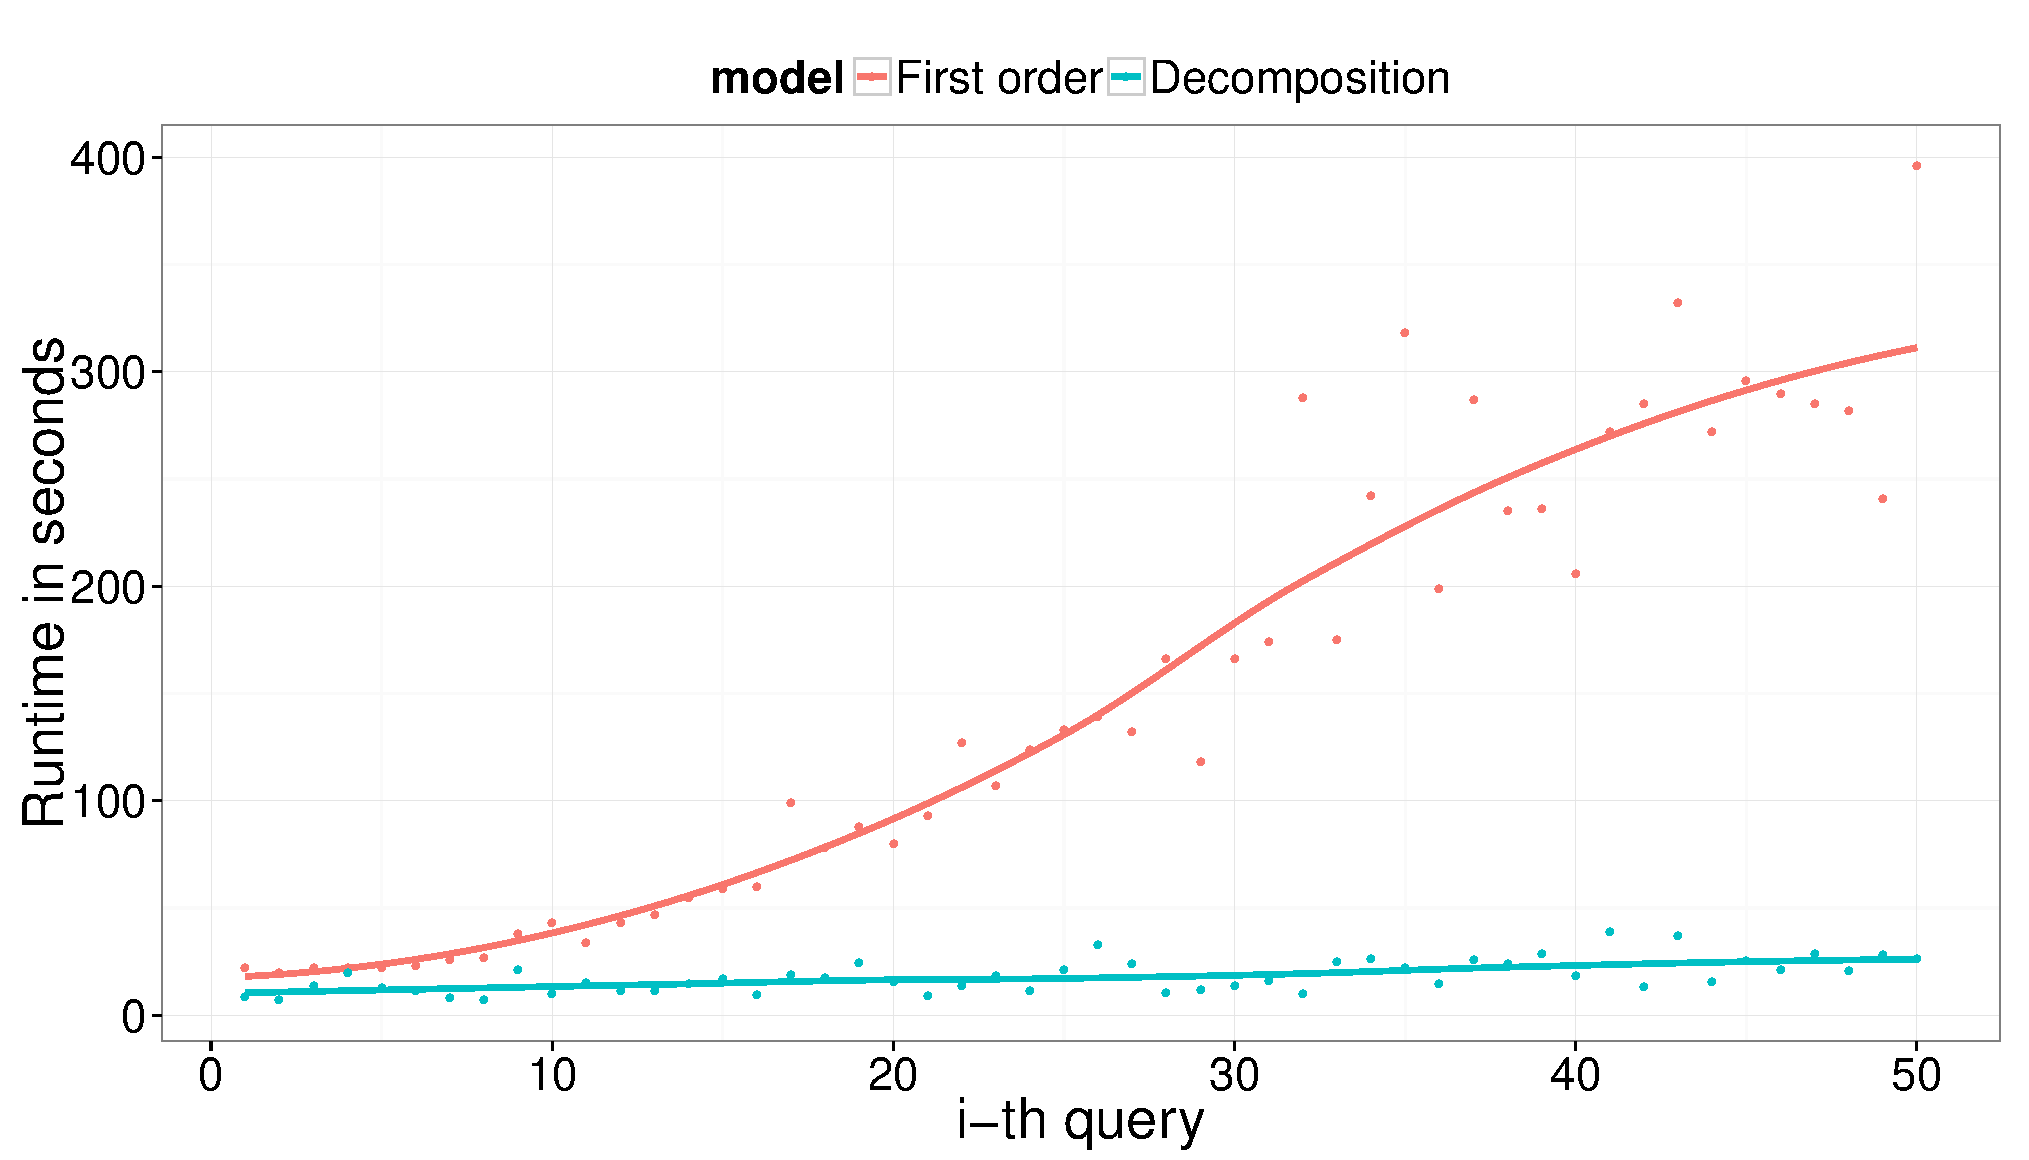
\includegraphics[scale=0.14]{extra/figure_comparison_yoshida.pdf}
\caption{\footnotesize{IDP model comparison: the disjoint union model has a steady growing trend while the higher order model stays flat. The average runtime gap is two orders of magnitude. (Due to \cite{ilp_graph_mining})}}
  \label{fig:decomposition_idp}
\end{subfigure}%
\hfill
\begin{subfigure}{0.46\textwidth}
  \centering
 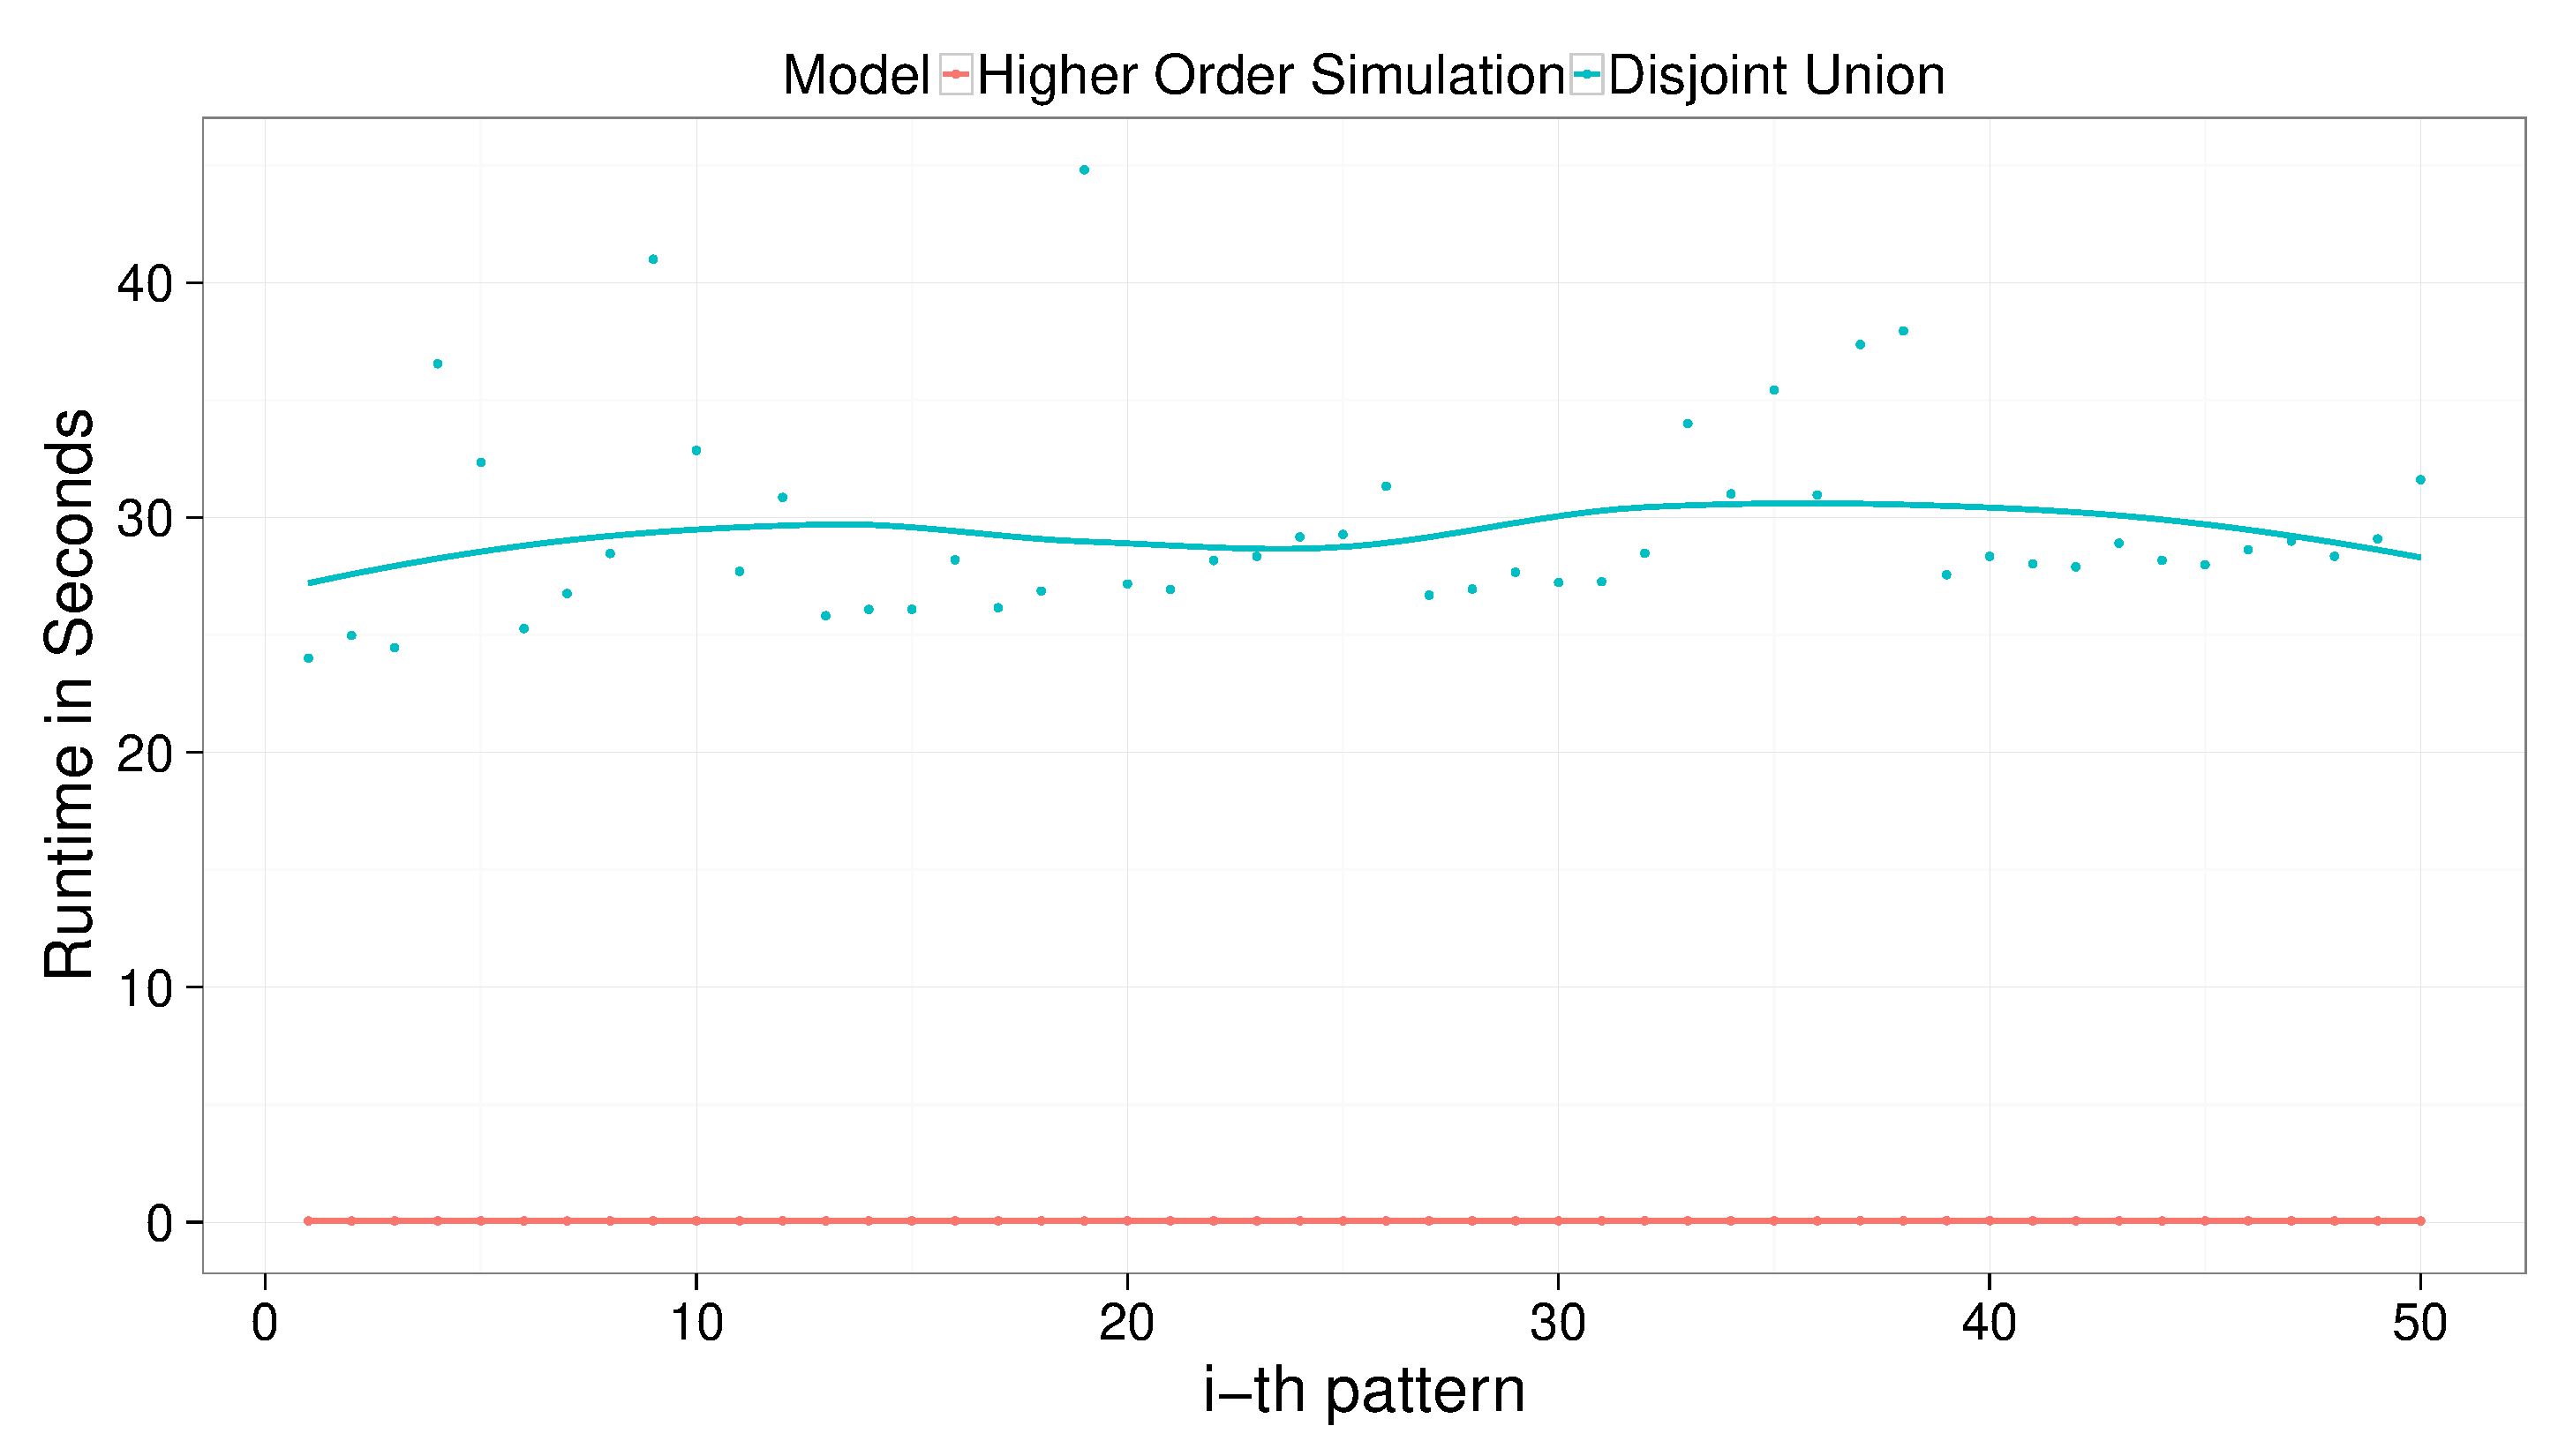
\includegraphics[scale=0.14]{extra/asp_fol_vs_decomposed_yoshida.pdf}
 \caption{\footnotesize{ASP model comparison: the disjoint union model exhibits fluctuation around the runtime of 30s, showing a slow runtime growth, while the higher order model stays flat. The runtime gap is two orders of magnitude.}}
  \label{fig:decomposition_asp}
\end{subfigure}
\caption{\footnotesize{Frequent graph enumeration problem (5\% frequency threshold) on Yoshida dataset \cite{yoshida_dataset} run on two systems IDP (a) and ASP (b), comparing disjoint union models (in red) and higher order simulations (in blue). For simulations we generated a candidate (levelwise from smaller to larger), checked frequency for individual patterns until we reach the threshold (for disjoint union this step is done in one call), then generated isomorphic no-goods, and repeated the process. Further explanations and the code can be found in the appendix.}}
\label{fig:decomposition_fol}
\end{figure}
